\chapter{System Design}
\label{System Design}
\section{Module Description}
	Module description focuses on detailed implementation of the system recommended in feasibility study. It is transition from user-oriented document to programmer-oriented document. In the Module description firstly identified the main objects and operations involved in the PC control. In the identification process, listed out main levels in module description that play major roles in this app:- android design, android coding, server and notification.
	In the next step, the key roles these objects are identified with relationship to each other. The user name and password of new user after successful registration process will store in the database. 
\section{Data Flow Diagrams}
\label{Data Flow Diagrams}
	A DFD, also known as a "Bubble Chart", has the purpose of clarifying system requirements and identifying major transformations that will become programs in system design. So it is the starting point of the design phase that functionally decomposes the requirements specifications down to the lowest level of detail.Data floe diagrams are made up of a number of symbols, which represent system components. Most data flow modelling models include four symbols which represent four  kinds of system components Processes, data stores, data flows and external 

\begin{figure}
entities. Below figures shows various levels of DFD's. User registration shown in figure 3.1, user login shown in figure 3.2, remote desktop access shown in figure 3.3, power option shown in figure 3.4, and send message shown in figure 3.5. 
\subsection{Level 1}
\label{Level 1}
\begin{center}
\scalebox{0.70}
%{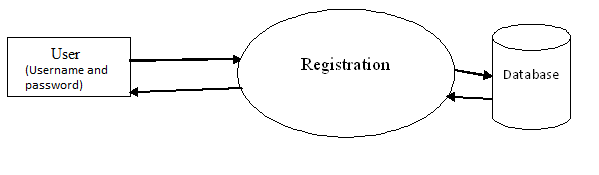
\includegraphics{login1.png}}
{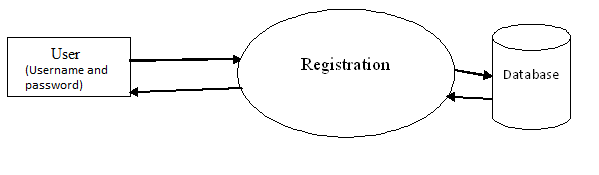
\includegraphics{login1.png}}
\caption{DFD-User Registration}
\end{center}
\end{figure}


\begin{figure}
\subsection{Level 2}
\label{Level 2}
\begin{center}
\scalebox{0.70}
%{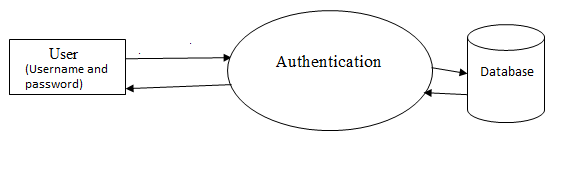
\includegraphics{login2.png}}
{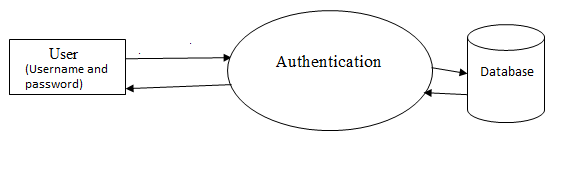
\includegraphics{login2.png}}
\caption{DFD-User Login}  
\end{center}
\end{figure}


\begin{figure}
\subsection{Level 3}
\label{Level 3} 
\begin{center}
\scalebox{0.70}
%{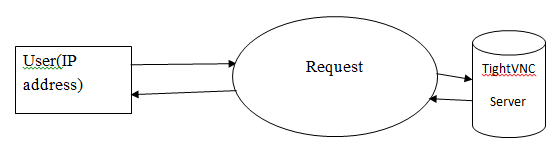
\includegraphics{f3.png}}
{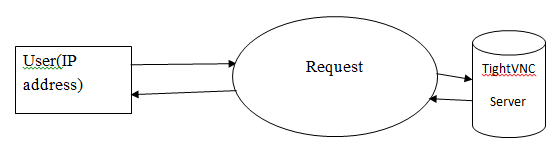
\includegraphics{f3.png}}
\caption{DFD-Remote Desktop Access} 
\end{center}
\end{figure}


\begin{figure}
\subsection{Level 4}
\label{Level 4}
\begin{center}
\scalebox{0.70}
%{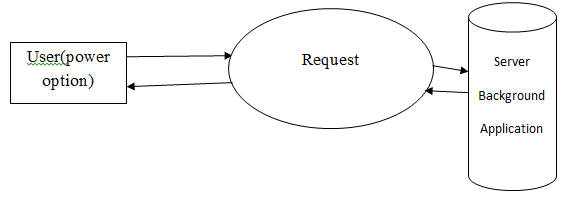
\includegraphics{power1.png}}
{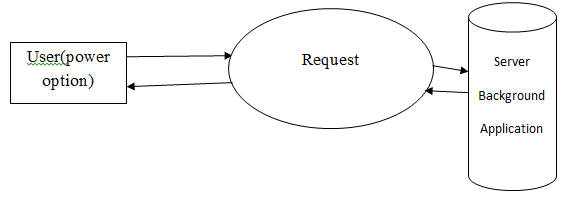
\includegraphics{power1.png}}
\caption{DFD-Power Options}  
\end{center}
\end{figure}


\begin{figure}
\subsection{Level 5}
\label{Level 5} 
\begin{center}
\scalebox{0.70}
%{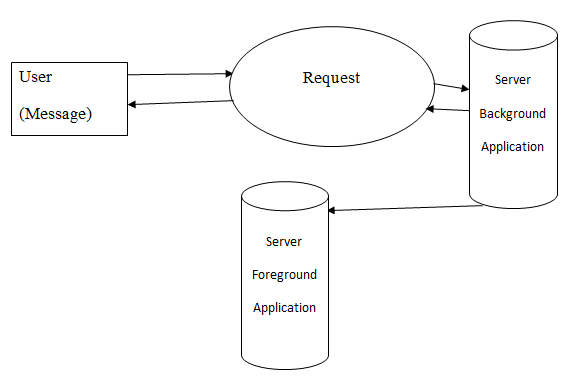
\includegraphics{send1.png}}
{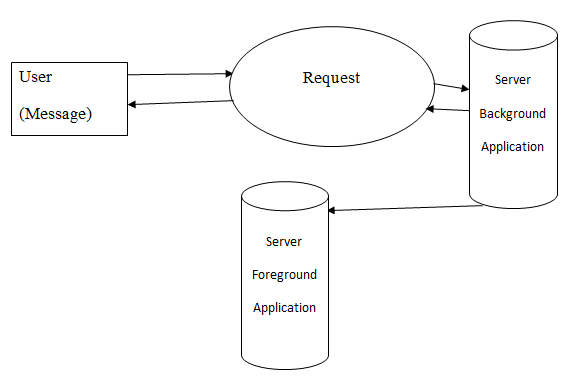
\includegraphics{send1.png}}
\caption{DFD-Send Message} 
\end{center}
\end{figure}	


